\section{Data Analysis}
\label{Analysis}
\subsection{Calculation of Angular Correlation}
The efficiency and acceptance of the neutron detector array varies greatly over the range of opening angles from 0 to 2$\pi$ (see figure~\ref{fig:OpeningAngleAcceptance}a).
This effect is due both to the detector array's non-spherical symmetry, and to varying efficiency as a function of particle position.
There was no attempt to measure the array's efficiency as a function of two-neutron opening angle, because this is not necessary and would have been a difficult task.
In this experiment, angular correlation is calculated by normalizing opening angle measurements to an equivalent distribution of uncorrelated neutrons, giving a result that is insensitive to detector efficiencies.
This effect is illustrated by the difference between figure~\ref{fig:OpeningAngleAcceptance}a and figure~\ref{fig:OpeningAngleAcceptance}b.
The equivalent uncorrelated distribution is formed from a set of manufactured two-neutron events, in which each neutron is taken from a different pulse and the opening angle between them calculated normally.
Such nuetron pairs will hereafter be referred to as different pulse (DP) pairs.
The neutrons of a DP pair are uncorrelated because events in one pulse do not have casual influence on the events in another pulse.
Detector efficiency and geometry influence same pulse (SP) events and DP events equally.\todo{ToDo: further explain why this statement holds true}
Thus, barring two-neutron correlations and a scaling factor, the DP distribution is identical to the SP distribution.
Each pair of pulses is chosen such that the two pulses occurred within less than a few 100 ms of each other.
This ensures that both pulses are subject to the same experimental conditions, thereby lessening systematic effects from time varying factors such as high-voltage drift and varying beam current.
As many pairs as needed can be readily selected until good counting statistics is achieved, because the only restriction for selecting pulse pairs is that they occurred around roughly the same time.
% ToDo: Compare our result for CF252 to another result. Overlay with this figure.
\begin{figure}
    \centering
    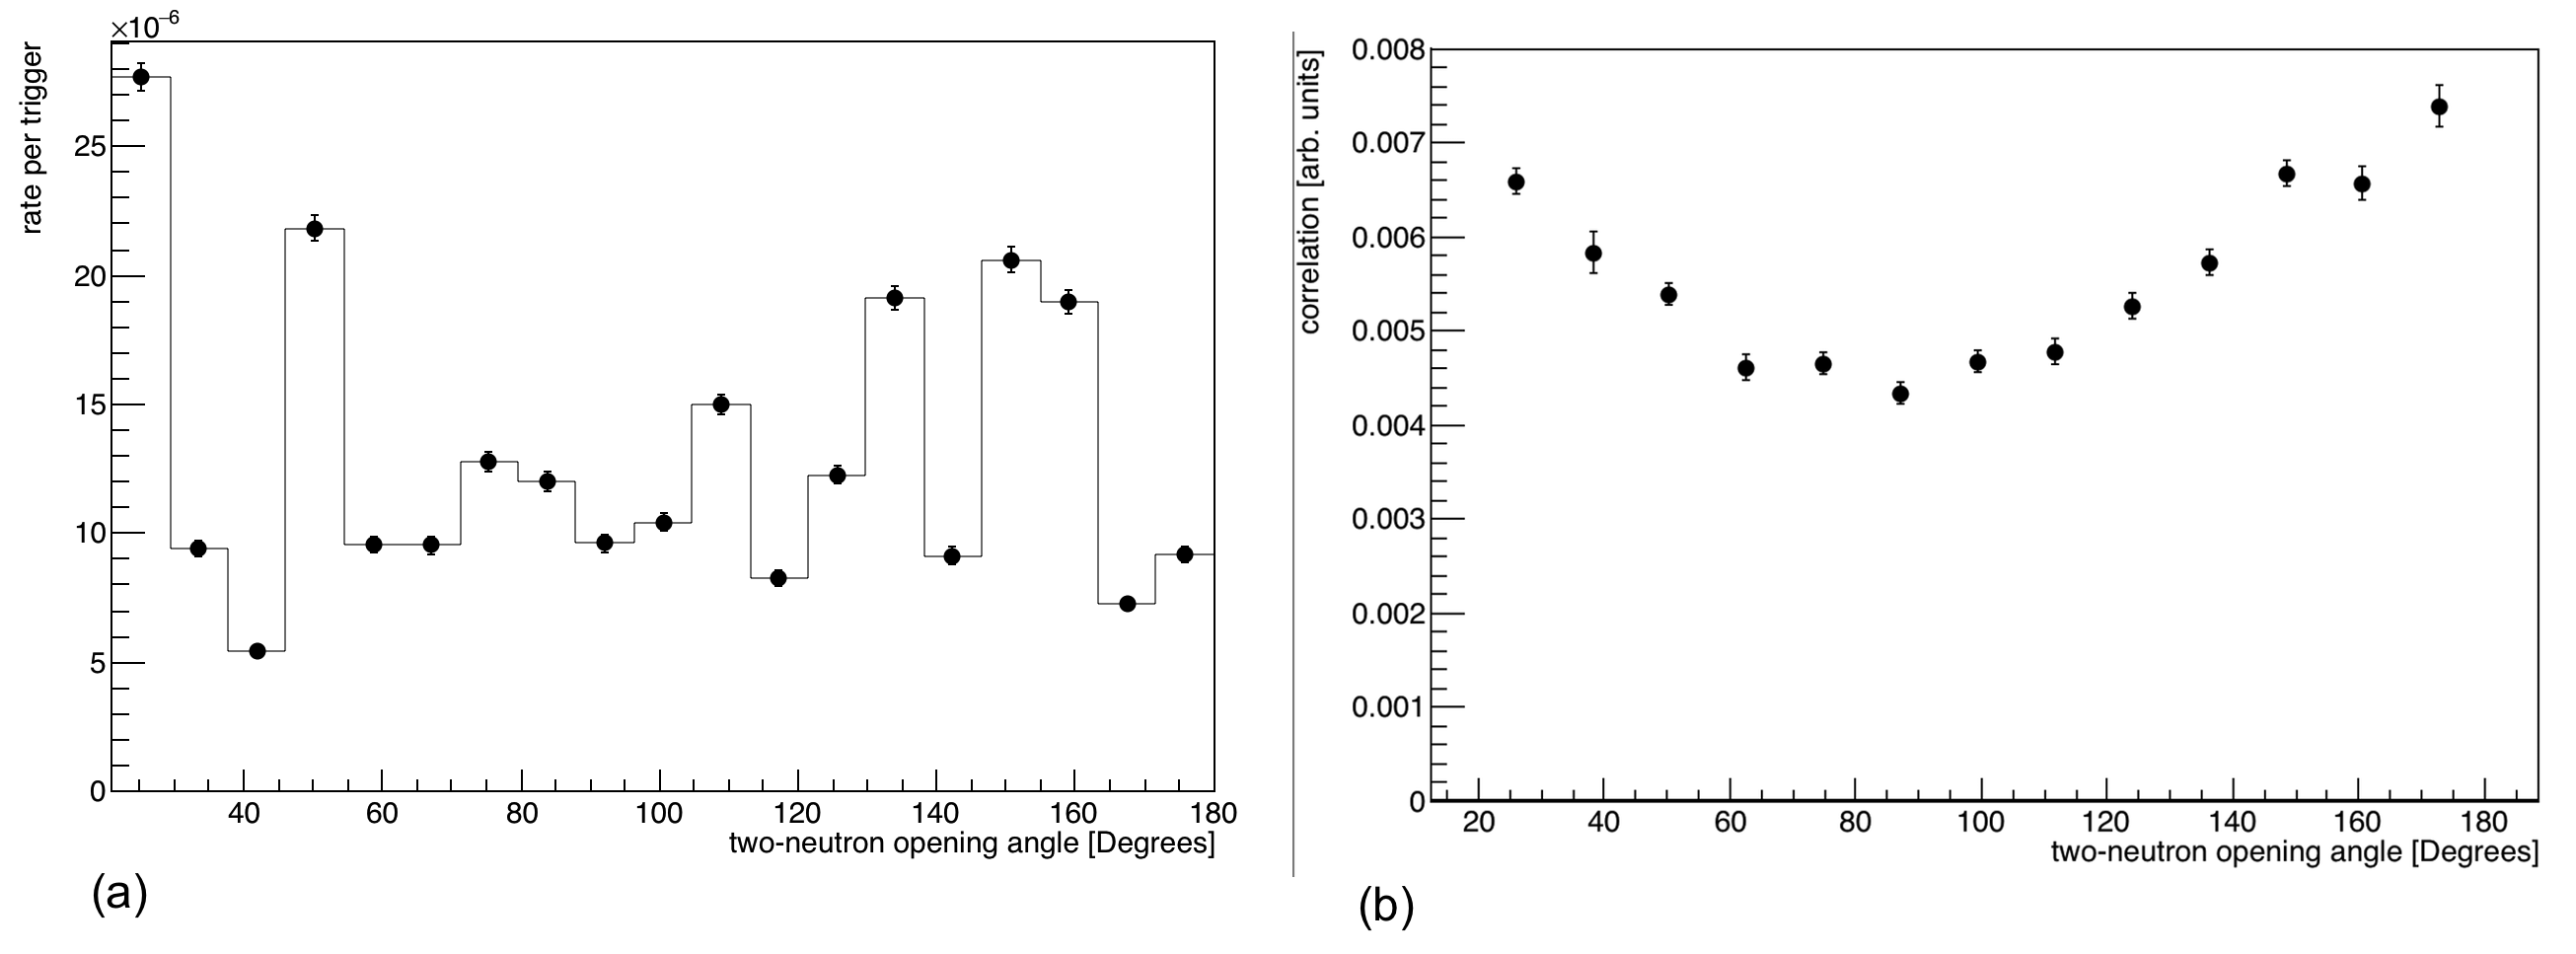
\includegraphics[width  = \textwidth ]{Content/Methods/Normalization.png}
    \caption{(a) Unnormalized two-neutron opening angle distribution from the spontaneous fission of $^{252}$Cf. The structure is reflective of geometric acceptance and efficiencies. (b) Same distribution after division by uncorrelated two-neutron events, which are taken from different pulses.}
    \label{fig:OpeningAngleAcceptance}
    \label{fig:OpeningAngleAcceptance}
\end{figure}

\subsection{Subtraction of Accidentals}
\label{Subtraction of Accidentals}
An accidental neutron coincidence is defined as a coincidence between two uncorrelated events in a single pulse.
For example, a coincidence between a neutron from a (gamma,1n) reaction and a neutron from photofission.
Another example is a coincidence between two events that are part of the noise background.
In both of these examples, the two events are considered accidentals because they have no causal influence on each another.
A true neutron coincidence, or true for short, is defined here as any pair correlated neutrons from the same pulse.

Accidentals are removed from the data by subtracting 1/2 times the equivalent distribution formed by the DP data.
The factor of 1/2 arises from the Poissonian statistics that inherently govern all accidentals, whether the accidental events are composed of two neutrons, two photons, two noise events, or any combination thereof\todo{ToDo: Explain why the use of Poissonian statistics is valid}.
An accidental is comprised of the occurrence of two independent events.
Therefore, as per Poissonian statistics, the probability of measuring an accidental in a single pulse is given by:
\begin{displaymath}
SP_{\text{a}} = \frac{e^{-\lambda}\lambda^2}{2} \approx \frac{1}{2}\lambda^{2}
\end{displaymath}
where $SP_{a}$ is the accidental rate of single pulses, $\lambda$ is the mean accidental rate of single pulses–an unknown value.
In this study, the coincidence rates were around $5\times10^{-5}$ events per pulse, so the approximation used above is correct to within 0.001\% as the worst case scenario.
Since the DP data is formed by observations of events from two different pulses, the DP accidental rate is equal to the poissonian probability of observing exactly one event, squared:
\begin{displaymath}
DP_{\text{a}} = (e^{-\lambda}\lambda)^{2}\approx \lambda^{2} 
\end{displaymath}
where $DP_{\text{a}}$ is the accidental rate of DP events.
Therefore, if coincidence rates, then the rate of measured accidentals in single pulses is 1/2 times the rate of accidentals in the different pulses.
In this study the subtraction had about a ten percent effect.
